\documentclass[uplatex, dvipdfmx, a4j,11pt]{jsarticle}
\usepackage[dvipdfmx]{graphicx}
\usepackage{lastpage}
\usepackage{fancyhdr}
\usepackage{listings}
\usepackage{jlisting}
\usepackage{xcolor}
\usepackage{url}

\makeatletter
\title{演習課題2}
\author{202310330 長田悠生}
\date{2024年5月18日}

\pagestyle{fancy}

\lstset{
    basicstyle = {\ttfamily}, % 基本的なフォントスタイル
    frame = {tbrl}, % 枠線の枠線。t: top, b: bottom, r: right, l: left
    breaklines = true, % 長い行の改行
    numbers = none, % 行番号の表示。left, right, none
    % stepnumber=1, % 行番号増分
    % numbersep=10pt, % 行番号と本文の間隔 デフォルト:10pt
    showspaces = false, % スペースの表示
    showstringspaces = false, % 文字列中のスペースの表示
    showtabs = false, % タブの表示
    keywordstyle = \color{blue}, % キーワードのスタイル。intやwhileなど
    commentstyle = {\color[HTML]{1AB91A}}, % コメントのスタイル
    identifierstyle = \color{black}, % 識別子のスタイル 関数名や変数名
    stringstyle = \color{brown}, % 文字列のスタイル
    captionpos = t % キャプションの位置 t: 上、b: 下
}

\lstdefinelanguage{Julia}
{
  keywordsprefix=\@,
  morekeywords={
    exit,whos,edit,load,is,isa,isequal,typeof,tuple,ntuple,uid,hash,finalizer,convert,promote,
    subtype,typemin,typemax,realmin,realmax,sizeof,eps,promote_type,method_exists,applicable,
    invoke,dlopen,dlsym,system,error,throw,assert,new,Inf,Nan,pi,im,begin,while,for,in,return,
    break,continue,macro,quote,let,if,elseif,else,try,catch,end,bitstype,ccall,do,using,module,
    import,export,importall,baremodule,immutable,local,global,const,Bool,Int,Int8,Int16,Int32,
    Int64,Uint,Uint8,Uint16,Uint32,Uint64,Float32,Float64,Complex64,Complex128,Any,Nothing,None,
    function,type,typealias,abstract
  },
  sensitive=true,
  morecomment=[l]{\#},
  morestring=[b]',
  morestring=[b]"
}
\renewcommand{\lstlistingname}{}

% headers & footers
\lhead{数値計算法 \@title 提出日:\@date\\\@author}
\chead{}
\rhead{}
\lfoot{}
\cfoot{\thepage/\pageref{LastPage}}
\rfoot{}
\renewcommand{\headrulewidth}{0pt}
\renewcommand{\footrulewidth}{0pt}
\makeatother

\begin{document}
\section*{課題1}
\subsection*{(1-1)}
\begin{lstlisting}[title={(1-1)のソースコード}, label=code:in, language=Julia]
module MonteCarloModule
    using Random
    Random.seed!(0)
    function MonteCarlo(n::Int64)::Float64
        x::Vector{Float64} = zeros(Float64, n)
        y::Vector{Float64} = zeros(Float64, n)
        for i::Int64 = 1:n
            x[i] = rand()
            y[i] = rand()
        end
        r::Vector{Float64} = zeros(Float64, n)
        for i::Int64 = 1:n
            r[i] = x[i]^2 + y[i]^2
        end
        m::Int64 = 0
        for i::Int64 = 1:n
            if r[i] <= 1
                m = m + 1
            end
        end
        p::Float64 = 4*m/n
        return p
    end

    function monte_carlo_func(n::Int64)::Float64
        if n <= 0
            throw("n have to larger than 0.")
        end
        return MonteCarlo(n)
    end
end

\end{lstlisting}

\newpage
\textmc{前ページの関数について具体的なnの値を入れてみたときのソースコードと出力結果です。前ページのソースコードと以下のソースコードは同一のファイルに書いています。}

\begin{lstlisting}[title={上記の関数に具体的なnの値を入れてみたときのソースコード}, label=code:in, language=Julia]
using .MonteCarloModule

p_1::Float64 = MonteCarloModule.monte_carlo_func(1)
println("p_1 = $p_1")

p_100::Float64 = MonteCarloModule.monte_carlo_func(100)
println("p_100 = $p_100")

p_0::Float64 = MonteCarloModule.monte_carlo_func(0)
println("p_0 = $p_0")

\end{lstlisting}

\begin{lstlisting}[title={実行結果}, label=code:in, language=sh]
$ julia --project ./src/report1-1.jl
p_1 = 4.0
p_100 = 3.28
ERROR: LoadError: "n have to larger than 0."
Stacktrace:
    [1] monte_carlo_func(n::Int64)
    @ Main.MonteCarloModule ~/Desktop/julia-numeric-calculation/class2_report/src/report1-1.jl:27
    [2] top-level scope
    @ ~/Desktop/julia-numeric-calculation/class2_report/src/report1-1.jl:41
in expression starting at /home/hello/Desktop/julia-numeric-calculation/class2_report/src/report1-1.jl:41

\end{lstlisting}

\newpage
\subsection*{(1-2)}
\begin{lstlisting}[title={(1-2)のソースコード}, label=code:in, language=Julia]
module MonteCarloModule
    using Random
    Random.seed!(0)
    function MonteCarlo(n::Int64)::Float64
        x::Vector{Float64} = zeros(Float64, n)
        y::Vector{Float64} = zeros(Float64, n)
        for i::Int64 = 1:n
            x[i] = rand()
            y[i] = rand()
        end
        r::Vector{Float64} = zeros(Float64, n)
        for i::Int64 = 1:n
            r[i] = x[i]^2 + y[i]^2
        end
        m::Int64 = 0
        for i::Int64 = 1:n
            if r[i] <= 1
                m = m + 1
            end
        end
        p::Float64 = 4*m/n
        return p
    end

    function monte_carlo_func(n::Int64)::Float64
        if n <= 0
            throw("n have to larger than 0.")
        end
        return MonteCarlo(n)
    end

    struct MonteCarloData
        n_vec::Array{Float64}
        result_vec::Array{Float64}
    end

    function monte_carlo_data_func(size::Int64)::MonteCarloData
        n_vec::Array{Int64} = zeros(Int64, size)
        result_vec::Array{Float64} = zeros(Float64, size)
        for i::Int64 = range(1, size, size)
            n::Int64 = 10^i
            result::Float64 = monte_carlo_func(n)
            n_vec[i] = n
            result_vec[i] = abs(result - pi)
        end
        data::MonteCarloData = MonteCarloData(n_vec, result_vec)
        return data
    end
end

using .MonteCarloModule
using Plots

data::MonteCarloModule.MonteCarloData = MonteCarloModule.monte_carlo_data_func(6)

plot(data.n_vec, data.result_vec, xaxis=:log)
savefig("report1-2.png")

\end{lstlisting}

\begin{figure}[h]
  \begin{center}
    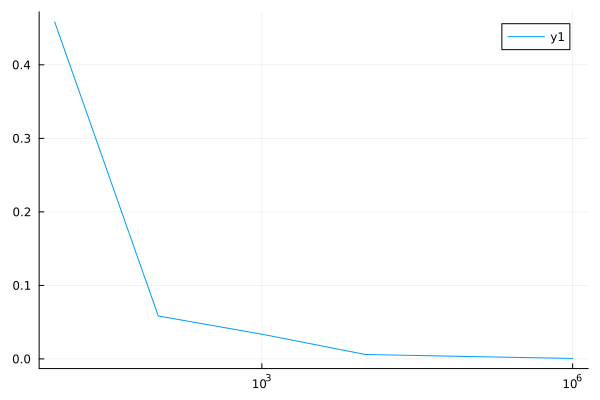
\includegraphics[width=120mm]{report1-2.png}
    \caption{実行結果のグラフ}
  \end{center}
\end{figure}

\newpage

\section*{課題2}
\subsection*{(2-1)}
\textmc{
    課題2では$roots(Polynomial([c, b, a]))$で計算した結果を正しいものと仮定しているので、
    $\frac{-b + \sqrt{b^2 -4ac}}{2a} = (-b + sqrt(b^2.0 -4.0*a*c))/(2.0*a)$、
    $\frac{-b - \sqrt{b^2 -4ac}}{2a} = (-b - sqrt(b^2.0 -4.0*a*c))/(2.0*a)$とすると、
    残差の計算式を$\Bigg|f\left(\frac{-b - \sqrt{b^2 -4ac}}{2a}\right) - 0 \Bigg|$と
    $\Bigg|f\left(\frac{-b + \sqrt{b^2 -4ac}}{2a}\right) - 0 \Bigg|$ではなく、
    $\Bigg|f\left(\frac{-b - \sqrt{b^2 -4ac}}{2a}\right) - f(roots(Polynomial([c, b, a]))[1]) \Bigg|$と
    $\Bigg|f\left(\frac{-b + \sqrt{b^2 -4ac}}{2a}\right) - f(roots(Polynomial([c, b, a]))[2]) \Bigg|$にしている。
}
\begin{lstlisting}[title={(2-1)のソースコード}, label=code:in, language=Julia]
    module QuadraticEquation
    using Polynomials

    struct Term
        c::Float64
        b::Float64
        a::Float64
    end

    struct Solution
        true_value::Array{Float64}
        approximation_value::Array{Float64}
    end

    function approximation_func(term::Term)::Array{Float64}
        return [(-term.b - sqrt(term.b^2.0 -4.0*term.a*term.c))/(2.0*term.a), (-term.b + sqrt(term.b^2.0 -4.0*term.a*term.c))/(2.0*term.a)]
    end

    function true_func(term::Term)::Array{Float64}
        coefficient::Array{Float64} = [term.c, term.b, term.a]
        return roots(Polynomial(coefficient))
    end

    function absolute_error_func(solution::Solution)::Array{Float64}
        return [
            abs(solution.true_value[1] - solution.approximation_value[1]),
            abs(solution.true_value[2] - solution.approximation_value[2])
        ]
    end

    function relative_error_func(solution::Solution)::Array{Float64}
        return [
            abs(solution.approximation_value[1] - solution.true_value[1]) / abs(solution.true_value[1]),
            abs(solution.approximation_value[2] - solution.true_value[2]) / abs(solution.true_value[2]),
        ]
    end

    function quadratic_equation(term::Term, x::Float64)::Float64
        return term.a*x^2 + term.b*x + term.c
    end

    function rest_func(term::Term, solution::Solution)::Array{Float64}
        return [
            abs(quadratic_equation(term, solution.approximation_value[1]) - quadratic_equation(term, solution.true_value[1])),
            abs(quadratic_equation(term, solution.approximation_value[2]) - quadratic_equation(term, solution.true_value[2])),
        ]
    end
end

import .QuadraticEquation

values::QuadraticEquation.Term = QuadraticEquation.Term(1.0, -124.0, 1.0)

println("===解の公式を使って解を求める===")
approximation_value::Array{Float64} = QuadraticEquation.approximation_func(values)
println(approximation_value)

println("===正確な解を求める===")
true_value::Array{Float64} = QuadraticEquation.true_func(values)
println(true_value)

solution::QuadraticEquation.Solution = QuadraticEquation.Solution(true_value, approximation_value)

println("===絶対誤差===")
absolute_error::Array{Float64} = QuadraticEquation.absolute_error_func(solution)
println(absolute_error)

println("===相対誤差===")
relative_error::Array{Float64} = QuadraticEquation.relative_error_func(solution)
println(relative_error)

true_result_1 = QuadraticEquation.quadratic_equation(values, solution.true_value[1])
true_result_2 = QuadraticEquation.quadratic_equation(values, solution.true_value[2])
approximation_result_1 = QuadraticEquation.quadratic_equation(values, solution.approximation_value[1])
approximation_result_2 = QuadraticEquation.quadratic_equation(values, solution.approximation_value[2])
println("===2次方程式の解を求める===")
println("x = $(solution.true_value[1]) のとき、")
println("$(values.a)*x^2 + $(values.b)*x + $(values.c) = $true_result_1")
println("x = $(solution.true_value[2]) のとき、")
println("$(values.a)*x^2 + $(values.b)*x + $(values.c) = $true_result_2")
println("x = $(solution.approximation_value[1]) のとき、")
println("$(values.a)*x^2 + $(values.b)*x + $(values.c) = $approximation_result_1")
println("x = $(solution.approximation_value[2]) のとき、")
println("$(values.a)*x^2 + $(values.b)*x + $(values.c) = $approximation_result_2")

println("===残差===")
rest_value = QuadraticEquation.rest_func(values, solution)
println(rest_value)

\end{lstlisting}

\newpage
\begin{lstlisting}[title={実行結果}, label=code:in, language=sh]
$ julia --project ./src/report2-1.jl
===解の公式を使って解を求める===
[0.008065040684527958, 123.99193495931547]
===正確な解を求める===
[0.008065040684526154, 123.99193495931547]
===絶対誤差===
[1.8041124150158794e-15, 0.0]
===相対誤差===
[2.2369538922194248e-13, 0.0]
===2次方程式の解を求める===
x = 0.008065040684526154 のとき、
1.0*x^2 + -124.0*x + 1.0 = 1.1102230246251565e-16
x = 123.99193495931547 のとき、
1.0*x^2 + -124.0*x + 1.0 = 0.0
x = 0.008065040684527958 のとき、
1.0*x^2 + -124.0*x + 1.0 = -2.2359891715950653e-13
x = 123.99193495931547 のとき、
1.0*x^2 + -124.0*x + 1.0 = 0.0
===残差===
[2.2370993946196904e-13, 0.0]

\end{lstlisting}

\subsection*{(2-2)}
\textmc{
    課題2では$roots(Polynomial([c, b, a]))$で計算した結果を正しいものと仮定しているので、
    $\alpha = \frac{-b + \sqrt{b^2 -4ac}}{2a}$、
    $\beta = \frac{c}{a \alpha}$とすると、
    残差の計算式を$\Bigg|f\left( \frac{-b - \sqrt{b^2 -4ac}}{2a} \right) - 0 \Bigg|$と
    $\Bigg|f\left(\frac{-b + \sqrt{b^2 -4ac}}{2a}\right) - 0 \Bigg|$ではなく、
    $\Bigg|f(\beta) - f(roots(Polynomial([c, b, a]))[1]) \Bigg|$と
    $\Bigg|f(\alpha) - f(roots(Polynomial([c, b, a]))[2]) \Bigg|$にしている。
}

\begin{lstlisting}[title={実行結果}, label=code:in, language=Julia]
module QuadraticEquation
    using Polynomials

    struct Term
        c::Float64
        b::Float64
        a::Float64
    end\fra

    struct Solution
        true_value::Array{Float64}
        approximation_value::Array{Float64}
    end

    function approximation_func(term::Term)::Array{Float64}
        return [(-term.b - sqrt(term.b^2.0 -4.0*term.a*term.c))/(2.0*term.a), (-term.b + sqrt(term.b^2.0 -4.0*term.a*term.c))/(2.0*term.a)]
    end

    function true_func(term::Term)::Array{Float64}
        coefficient::Array{Float64} = [term.c, term.b, term.a]
        return roots(Polynomial(coefficient))
    end

    function absolute_error_func(solution::Solution)::Array{Float64}
        return [
            abs(solution.true_value[1] - solution.approximation_value[1]),
            abs(solution.true_value[2] - solution.approximation_value[2])
        ]
    end

    function relative_error_func(solution::Solution)::Array{Float64}
        return [
            abs(solution.approximation_value[1] - solution.true_value[1]) / abs(solution.true_value[1]),
            abs(solution.approximation_value[2] - solution.true_value[2]) / abs(solution.true_value[2]),
        ]
    end

    function quadratic_equation(term::Term, x::Float64)::Float64
        return term.a*x^2 + term.b*x + term.c
    end

    function rest_func(term::Term, solution::Solution)::Array{Float64}
        return [
            abs(quadratic_equation(term, solution.approximation_value[1]) - quadratic_equation(term, solution.true_value[1])),
            abs(quadratic_equation(term, solution.approximation_value[2]) - quadratic_equation(term, solution.true_value[2])),
        ]
    end

    function prevent_digit_loss_func(term::Term)::Array{Float64}
        alpha::Float64 = (-term.b + sqrt(term.b^2.0 -4.0*term.a*term.c))/(2.0*term.a)
        beta::Float64 = term.c / (alpha * term.a)
        return [beta, alpha]
    end

end

import .QuadraticEquation

values::QuadraticEquation.Term = QuadraticEquation.Term(1.0, -124.0, 1.0)

println("===桁落ちを防いで解を求める===")
prevent_digit_loss::Array{Float64} = QuadraticEquation.prevent_digit_loss_func(values)
println(prevent_digit_loss)

println("===正確な解を求める===")
true_value::Array{Float64} = QuadraticEquation.true_func(values)
println(true_value)

prevent_digit_loss_solution::QuadraticEquation.Solution = QuadraticEquation.Solution(true_value, prevent_digit_loss)

println("===絶対誤差===")
prevent_digit_loss_absolute_error::Array{Float64} = QuadraticEquation.absolute_error_func(prevent_digit_loss_solution)
println(prevent_digit_loss_absolute_error)

println("===相対誤差===")
prevent_digit_loss_relative_error::Array{Float64} = QuadraticEquation.relative_error_func(prevent_digit_loss_solution)
println(prevent_digit_loss_relative_error)

true_result_1 = QuadraticEquation.quadratic_equation(values, true_value[1])
true_result_2 = QuadraticEquation.quadratic_equation(values, true_value[2])
prevent_digit_loss_result_1 = QuadraticEquation.quadratic_equation(values, prevent_digit_loss[1])
prevent_digit_loss_result_2 = QuadraticEquation.quadratic_equation(values, prevent_digit_loss[2])
println("===2次方程式の解を求める===")
println("x = $(true_value[1]) のとき、")
println("$(values.a)*x^2 + $(values.b)*x + $(values.c) = $true_result_1")
println("x = $(true_value[2]) のとき、")
println("$(values.a)*x^2 + $(values.b)*x + $(values.c) = $true_result_2")
println("x = $(prevent_digit_loss[1]) のとき、")
println("$(values.a)*x^2 + $(values.b)*x + $(values.c) =  $prevent_digit_loss_result_1")
println("x = $(prevent_digit_loss[2]) のとき、")
println("$(values.a)*x^2 + $(values.b)*x + $(values.c) =  $prevent_digit_loss_result_2")

println("===残差===")
prevent_digit_loss_rest_value = QuadraticEquation.rest_func(values, prevent_digit_loss_solution)
println(prevent_digit_loss_rest_value)

\end{lstlisting}

\begin{lstlisting}[title={実行結果}, label=code:in, language=sh]
$ julia --project ./src/report2-2.jl
===桁落ちを防いで解を求める===
[0.008065040684526154, 123.99193495931547]
===正確な解を求める===
[0.008065040684526154, 123.99193495931547]
===絶対誤差===
[0.0, 0.0]
===相対誤差===
[0.0, 0.0]
===2次方程式の解を求める===
x = 0.008065040684526154 のとき、
1.0*x^2 + -124.0*x + 1.0 = 1.1102230246251565e-16
x = 123.99193495931547 のとき、
1.0*x^2 + -124.0*x + 1.0 = 0.0
x = 0.008065040684526154 のとき、
1.0*x^2 + -124.0*x + 1.0 =  1.1102230246251565e-16
x = 123.99193495931547 のとき、
1.0*x^2 + -124.0*x + 1.0 =  0.0
===残差===
[0.0, 0.0]

\end{lstlisting}

\subsection*{(2-3)}
\textmc{
  桁落ちは、絶対値が近い大きさの小数同士の減算を行ったときに、
  有効数字が減る減少である。桁落ちを防ぐ計算をしない場合でも
  $\frac{-b + \sqrt{b^2 -4ac}}{2a}$では誤差が生じておらず、
  $\frac{-b - \sqrt{b^2 -4ac}}{2a}$で誤差が生じているため、
  $-b$と$\sqrt{b^2 -4ac}$との減算で桁落ちが発生したと考えられる。
  また、桁落ちは絶対値が近い大きさの小数同士の減算を行ったときに有効数字が減るので、
  $|-b|$と$|\sqrt{b^2 -4ac}|$の大きさが近いと桁落ちが発生する。
  従って、$b^2$と$4ac$との差がとても大きいときに桁落ちが発生する可能性があると考えられる。
}

\begin{thebibliography}{9}
  \bibitem{julia} Chapter 8: Handling errors、Learn Julia the Hard Way \url{https://scls.gitbooks.io/ljthw/content/_chapters/11-ex8.html}
  \bibitem{julia} Juliaを基礎からゆっくりと(その08/18)、Hatena Blog \url{https://power-of-awareness.com/entry/2022/10/17/120000}
  \bibitem{julia} 【Julia】 基礎: 型、Qiita \url{https://qiita.com/Krypf/items/145ad24911ca51117e29}
  \bibitem{julia} Juliaの型定義、Qiita \url{https://qiita.com/bonten999/items/4fa3723884a5684c464c}
  \bibitem{julia} いまから使えるJulia言語、Julia in Physics 2021 Online \url{https://bicycle1885.org/slides/2021/juliainphysics2021/}
  \bibitem{latex} コンピュータソフトウェアのLaTeXスタイルファイルでlstlistingのキャプションが崩れる問題、Zenn \url{https://zenn.dev/niyaton/articles/9fa4daaab48d16}
  \bibitem{julia} JuliaでPlotsのグラフが表示されない、teratail \url{https://teratail.com/questions/366881}
  \bibitem{julia} 早わかり すぐに使える julia 1.0、早わかり すぐに使える julia 1.0 \url{https://cheatsheet.juliadocs.org/ja/}
  \bibitem{julia} Julia早引きノート[01]変数・定数の使い方、Qiita \url{https://qiita.com/ttabata/items/a1ada2c0cba03672e105}
  \bibitem{cancellation_of_significant_digits} 桁落ち、ZDNET \url{https://japan.zdnet.com/glossary/exp/%E6%A1%81%E8%90%BD%E3%81%A1/?s=4}
  \bibitem{cancellation_of_significant_digits} title、IT用語辞典e-Words \url{https://e-words.jp/w/%E6%A1%81%E8%90%BD%E3%81%A1.html}
  \bibitem{latex} chi-feng/preamble、GitHub \url{https://gist.github.com/chi-feng/6589066}
  \bibitem{latex} 【LaTeX】ソースコードの張り付け方、お茶の葉 \url{https://www.ochappa.net/posts/latex-code-b}
  \bibitem{latex} listings (download here) 、xyoshiki.web \url{http://xyoshiki.web.fc2.com/tex/listings.html}
  \bibitem{latex} Comprehensive TeX Archive Network、CTAN \url{https://www.ctan.org/tex-archive/macros/latex/contrib/listings}
  \bibitem{latex} LaTexに日本語を含むソースコードの記載、Qiita \url{https://qiita.com/izayoi5776/items/67a65dae5f2ce5ff84a3}
  \bibitem{latex} Latexに日本語を含んだソースコードを載せる、Hatena Blog \url{https://contents-open.hatenablog.com/entry/2021/07/24/140759}
  \bibitem{latex}LaTeX の Listing 対応言語一覧 、晴耕雨読 \url{https://tex2e.github.io/blog/latex/listing-predefined-languages}
\end{thebibliography}


\end{document}
